\documentclass[a4paper,ngerman]{scrartcl}

\usepackage{amsmath}
\usepackage{amsfonts}
\usepackage{amssymb}
\usepackage[utf8]{inputenc}
\usepackage{graphicx}
\usepackage[ngerman]{babel}
\usepackage{hyperref}
\usepackage{float}
\usepackage{caption}
\usepackage{subcaption}
\usepackage{multirow}  %for tables
\usepackage{icomma} % Handle german comma as decimal point in numbers
\usepackage{units,siunitx} % Write units with correct spacing
\usepackage{upgreek} % provide non-italic greek letters
\usepackage{url}
\usepackage{extpfeil}
%\usepackage{subfig}

% Formatting of table & figure captions
\captionsetup{font={sf,footnotesize},labelfont=bf,textfont=sl,skip=6pt}
\setlength{\abovecaptionskip}{6pt}
\setlength{\belowcaptionskip}{0pt}

\title{Black Lipid Membrane (BLM)}
\date{\today}
\author{Michel Rausch, Michael Eliachevitch}

\begin{document}

\maketitle
\tableofcontents
\newpage

\section{Einleitung}

In diesem Versuch werden Ionenkanäle in planaren Lipidmembranen untersucht. Hierbei wird der Wirkmechanismus des Antibiotikums Gramacidin A untersucht. In einer biologischen Zelle gelangen durch die entstandenen Kanäle Kationen durch die Zellmembran. Die Zelle stirbt aufgrund der Zerstörung ihres elektrochemischen Gradients [\ref{ref:mappe}].

Gramicidin beschreibt eine Gruppe Antibiotika. Dieses ist kommerziell unter Namen wie Angidin\textregistered , Mycolog\textregistered , Topsym\textregistered , Neospiron\textregistered  verfügbar. 


\section{Theoretische Grundlagen}

Die chemischen Grundlagen werden hier nicht genau behandelt. Gramicidin A1 besitzt die Summenformel $C_{99}H_{140}N_{20}O_{17}$. Es kann in der Natur von erdlebenden Bakterien beobachtet, aber auch synthetisch hergestellt werden. Mehrere Strukturen sind möglich, wobei Gramicidin A die häufigste ist. Gramicidin besitzt eine zyklische Struktur und damit einen anderen Wirkmechanismus. In diesem Experiment wird lediglich die Variante A verwendet.

\subsection{Wirkmechanismus}

Es existieren verschiedene Modelle, die Beschreiben, wie Gramicidin A in die Zellmembran integriert wird. Diese sind in Abbildung \ref{fig:wirkmechanismus} gezeigt. Auf die Einzelheiten wird nicht im Detail eingegangen.
\begin{itemize}
\item \textbf{A: Barrel Stave model} 
Hydrophobe, helixförmige Monomere bilden Poren in der Zellmembran.
\item \textbf{B: Toroidial Wormhole}  
Poremformation nahe phosphatidylethanolamine, oder phosphatidylserine Membranen. 
\item \textbf{C: Carpet model}  
Teppich-(engl. carpet-)ähnliche Anlagerung auf Membran.
\item \textbf{D} Detergent similar model
Bi- und Mizellen bilden Flächen auf der Membran. Durch deren Amphiphilie wird die Membran durchlässig.
\item \textbf{E} In-plane diffusion model
Verdünnung der Lipidschicht.
\end{itemize}

\begin{figure}
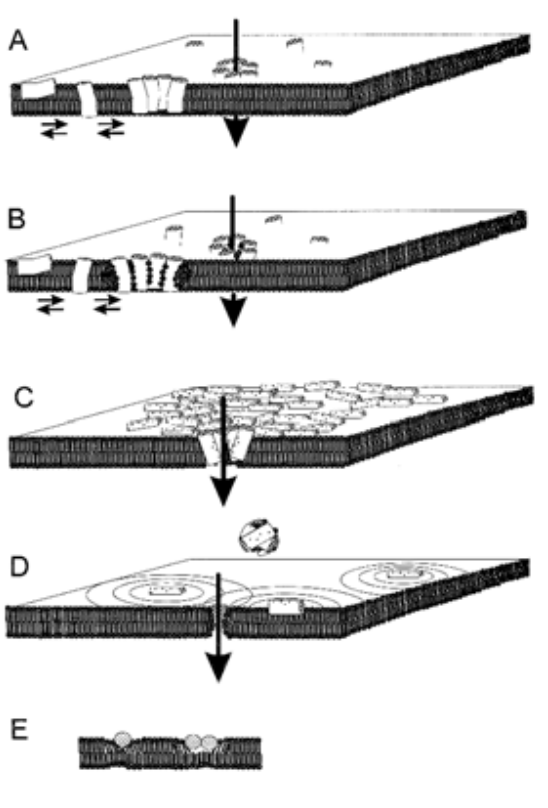
\includegraphics[width=0.5\textwidth]{abbildungen/wirkmechanismus.png}
\caption{Verschiedene Modelle zur Erklärung der Zerstörung einer Bakterienzelle mittels Peptid-Antibiotika [\ref{ref:mappe}]}
\label{fig:wirkmechanismus}
\end{figure}


\subsection{Ionentransport}

Eine Membran trennt zwei Bereiche einer wässrigen Lösung. Um sie zu überwinden, muss ein Ion eine Energie $E$ aufbringen. Die  Wahrscheinlichkeit k, eines Ions mit der Temperatur T, diese n einer Zeiteinheit zu überwinden ist der Ratenkoeffizient
\begin{equation} \label{eqn:rate}
k = k_0 e^{-\frac{E}{k_B T}},
\end{equation}
mit der Boltzmannkonstante $k_{B}$. Das Potential einer Membran lässt sich wie in Abbildung \ref{fig:potential-einfach} vorstellen. Die Ionen können in der Membran Bindungen eingehen, daher entstehen weitere Minima.

\begin{figure}
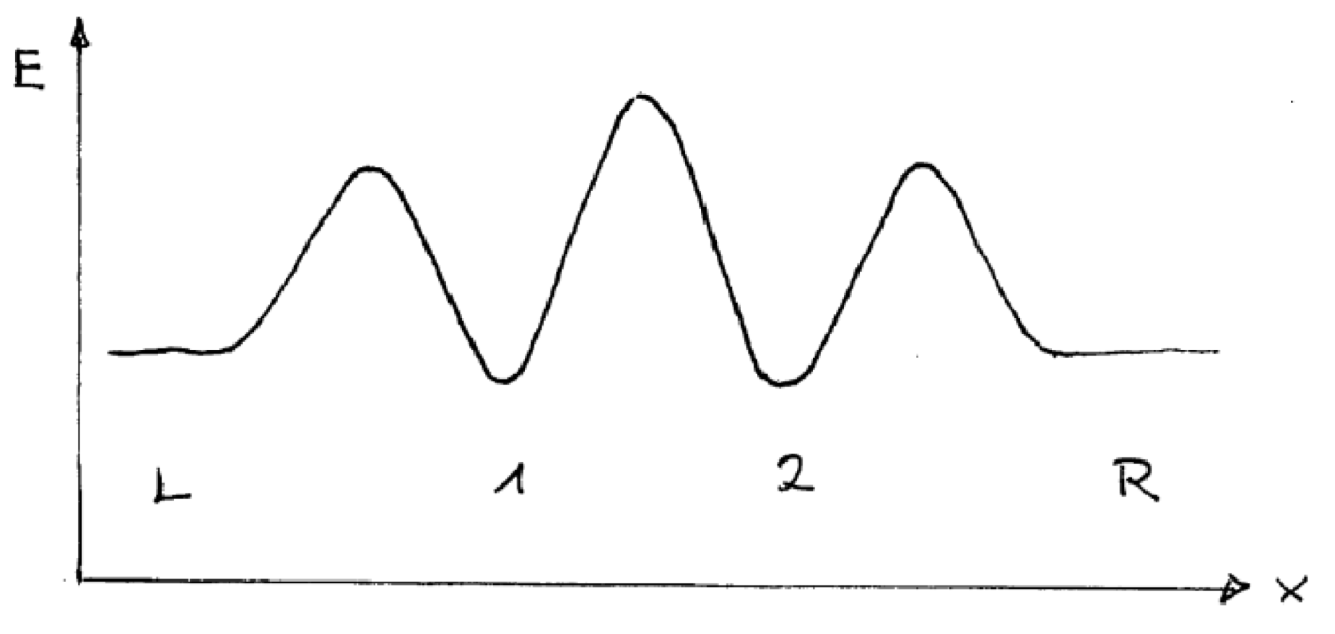
\includegraphics[width=0.6\textwidth]{abbildungen/potential-einfach.png}
\caption{Schema eines Potentials einer Pore [\ref{ref:mappe}]}
\label{fig:potential-einfach}
\end{figure}


Die Gleichung \ref{eqn:rate} wird auf den Fall des Experiments erweitert. Durch die angelegte Spannung $V_{m}$ wird das Potential asymmetrisch, wie in Abbildung \ref{fig:potential-asym} gezeigt.  Es wird die Quasistationaritätsnäherung verwendet. Die Leitfähigkeit eines einzelnen Kanals ist dann

\begin{equation}
\Lambda = \frac{k_A}{k_D} \cdot \frac{c}{k_A^{-1}+k^{-1}+k_D^{-1}} \cdot  \frac{q^2}{k_B T} .
\end{equation}

Mit der Ladung q der Ionen und den Ratenkoeffizienten $k_A$, $k_D$ und $k$ der Membran.
Hieraus ergeben sich die Zusammenhänge der makroskopisch Messbaren Größen

\begin{equation}
I_M = \lambda_M \cdot V_m
\end{equation}
und
\begin{equation}\label{eqn:transport-leitfaehigkeit}
\lambda_m = \Lambda \cdot N_p.
\end{equation}

Hierbei ist $I_M$ der gemessene Gesamtstrom an der Membran. $\lambda_M$ beschreibt die Leitfähigkeit der Membran.


\begin{figure}
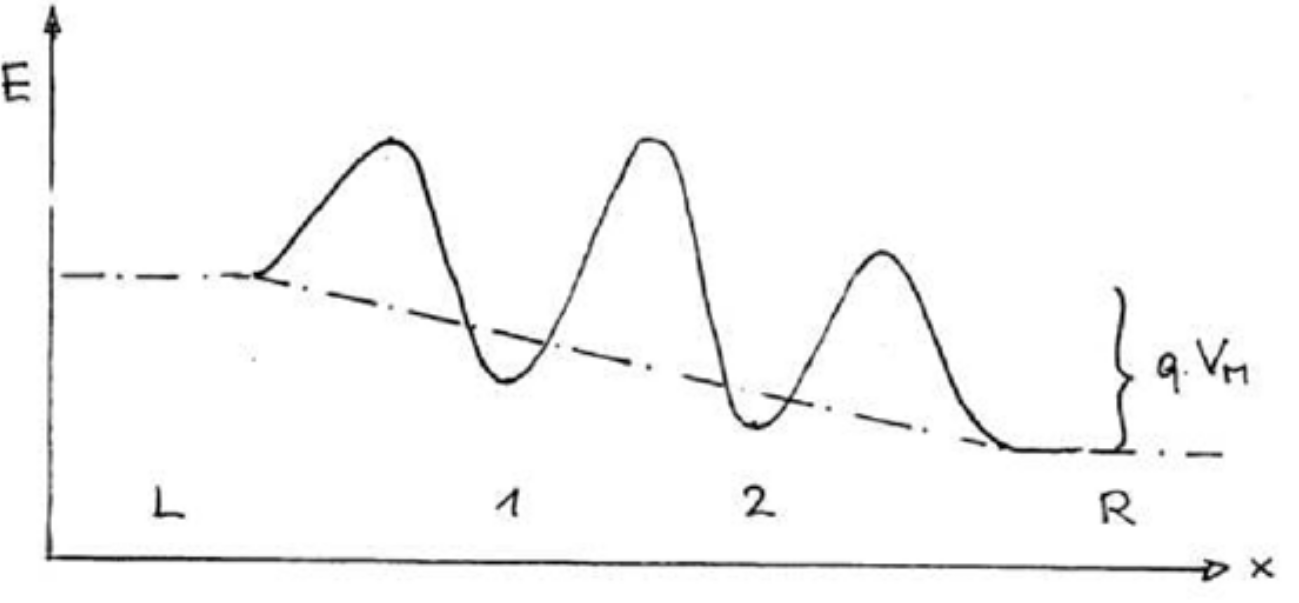
\includegraphics[width=0.6\textwidth]{abbildungen/potential-asym.png}
\caption{Schema des Potentials einer Pore mit angelegter Spannung [\ref{ref:mappe}]}
\label{fig:potential-asym}
\end{figure}



\subsubsection{Einzelkanalentstehung}

Nur Dimere des Gramicidin A führen zu einer Bildung von Ionenkanälen. Im Gleichgewicht werden Dimere gebildet und vernichtet. Dies führt zu einer variierenden Anzahl an Poren in der Membran und somit zu einer Fluktuation der Leitfähigkeit. Bei einer geringen Konzentration sind nur einzelne Kanäle vorhanden, daher ist die Quantisierung des Stromes $I_M$ deutlich erkennbar.

Die Dimerasation kann durch die Gleichung

\begin{equation}
G_1 + G_1 	\xtofrom[k_d]{k_r} G_2
\end{equation}

beschrieben werden. $k_d$ ist hier die Rate der Dissoziation und $k_r$ die der Entstehung der Dimere, $G_1$ entspricht den Monomeren, $G_2$ den Dimeren. Die Dissoziation folgt einem exponentiellem Zerfallsgesetz, die der Entstehungreaktion ist linear zum Quadrat der Konzentration. Aus dem Verlauf des Stromes über die zeit lässt sich die Zerfallsrate bestimmen.



\subsubsection{Mehrkanalentstehung}

Bei hohen Konzentrationen sind einzelne Kanäle nicht mehr ohne weiteres zu beobachten. Es gibt jedoch ein Rauschen in der Strommessung. Dies entstammt dem Öffnen und schließen von Kanälen. 
Die Reaktionsgleichung ergibt sich als
\begin{equation}\label{eqn:mehrkanal-reaktion1}
\frac{dG_2}{dt} = - k_d \cdot G_2 + k_r \cdot G_1^2 .
\end{equation}
Woraus folgt:
\begin{equation}\label{eqn:mehrkanal-reaktion2}
\frac{G_2}{G_1^2} = \frac{k_r}{k_d} .
\end{equation}

Die Gesamtzahl der Moleküle ist
\begin{equation}
G = G_1 + 2 \cdot G_2.
\end{equation}

Dieser Prozess kann beobachtet werden, wenn das Gleichgewicht, zum Beispiel mit einem elektrischem Feld, oder Temperaturänderung, gestört wird. 
Auch spontane Änderungen der Teilchenzahl können im Rauschen beobachtet werden.

Die Relaxationszeit ergibt sich aus Gleichungen \ref{eqn:mehrkanal-reaktion1} und \ref{eqn:mehrkanal-reaktion2}, zusammen mit \ref{eqn:transport-leitfaehigkeit} (mit $G_2 = N_P$) als

\begin{equation}
\tau^{-1} = k_d + 4 \cdot k_r \cdot G_1 = k_d + 4 \sqrt{\frac{k_d \cdot k_r}{\Lambda}  \cdot \lambda_M} .
\end{equation}

Deutlich zu erkennen ist die inverse wurzelförmige Abhängigkeit zur Leitfähigkeit

\subsubsection{Autokorrelationsfunkion}

Eine Autokorrelationsfunktion beschreibt die Korrelation eines Signals mit sich selbst zu einem früherem Zeitpunkt. 





\subsubsection{Charakteristik einer Membran}






\section{Versuchsaufbau}

\begin{figure}[tb!]
  \centering
  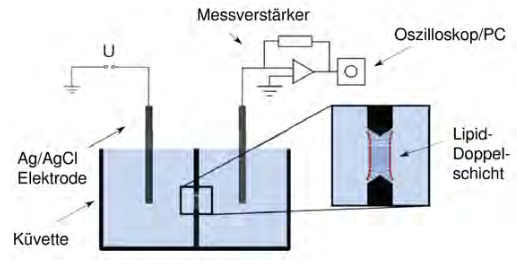
\includegraphics[width=0.9\textwidth]{abbildungen/blmaufbau.png}
  \caption{\textbf{Aufbau einer BLM ("`Black Lipid Membrane"').} \\Eine Küvette ist durch eine hydrophobe Trennwand zweigeteilt. Diese Trennwand hat ein kleines Loch in der Größenordnungen von Mikrometern, auf das die BLM "`aufgemalt"' ist. Die Küvette enthält eine Lösung und zwischen beiden Hälften kann durch Dioden eine Gleich- oder Wechselspannung angelegt werden. An einem Oszilloskop kann der Strom zwischen beiden Hälften beobachtet werden.}
  \label{fig:blmaufbau}
\end{figure}






\section{Aufgabenstellung und Versuchsdurchführung}

\subsection{Vorbereitung der Lipid-Doppelschicht}
\label{sec:bilayer-vorbereitung}

\subsection{Messung der Membran-Kapazität}
\label{sec:capacity}

\subsection{Messung einzelne Ionenkanäle}
\label{sec:singlechannels}

\subsection{Messung multipler Ionenkanäle}
\label{sec:multiplechannels}


\subsection{Noise-Analyse und Autokorrelationsfunktion}
\label{sec:noise-autocorr}

\subsection{Weitere Fragen}
\label{sec:weitere-fragen}















\section{Quellen}
\begin{enumerate}
\item Vorbereitungsmappe \label{ref:mappe}
\item pharmawiki.ch (16.11.2014) \label{ref:pharmawiki}
\end{enumerate}



\end{document}
